\section{Intalação}

%============================
\subsection{Visual Studio Code (VSCode)}

\tab
Primeiramente deve-se baixar e instalar o editor de código 
\href{https://code.visualstudio.com/}{Visual Studio Code},
pois é um ambiente mais amigável com o usuário e essencial
para utilizar as ferramentas necessárias para programar e configurar
o ESP32. Após instalar o VSCode, ao abri-lo entrará 
na página de \textit{Home} como na Figura \ref{fig:VSCodeHome}.

\begin{figure}[!ht]
    \centering
    \caption{Página Inicial ao abrir o VSCode}
    \vspace{0.2cm}
    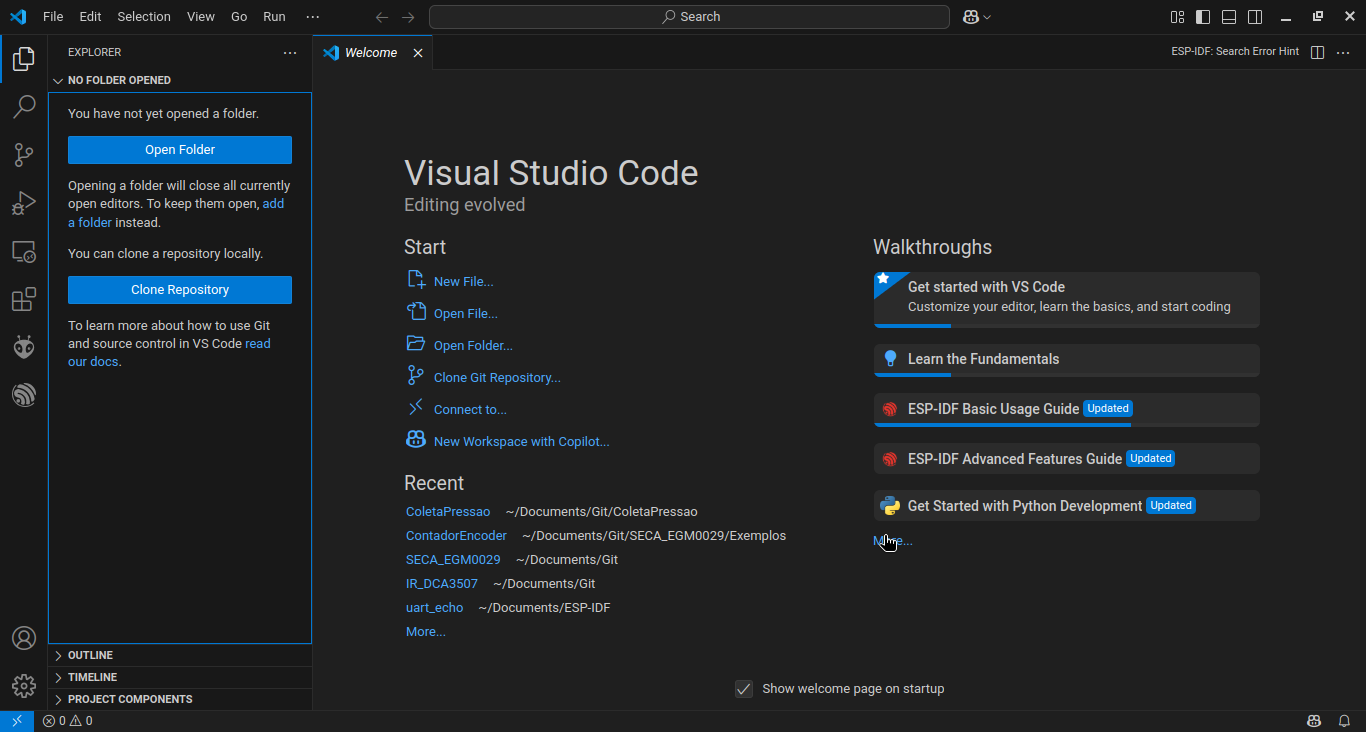
\includegraphics[scale=0.2]{img/VSCodeHome.png}
    \label{fig:VSCodeHome}
\end{figure}

%============================
\subsection{Extensão ESP-IDF}

\tab
No \textit{Home}, acesse a aba de \textbf{Extensões} na barra
de tarefas localizada na lado esquerdo da tela e pesquisa
pela extensão \textbf{ESP-IDF}, aparecerá uma janela parecido
como a Figura \ref{fig:VSCodeESPIDF}. Basta somente instalar a
extensão que aparecerá uma janela pedindo ao usuário configurar
a ESP-IDF no computador.

\begin{figure}[!ht]
    \centering
    \caption{Extensão da ESP-IDF no VSCode}
    \vspace{0.2cm}
    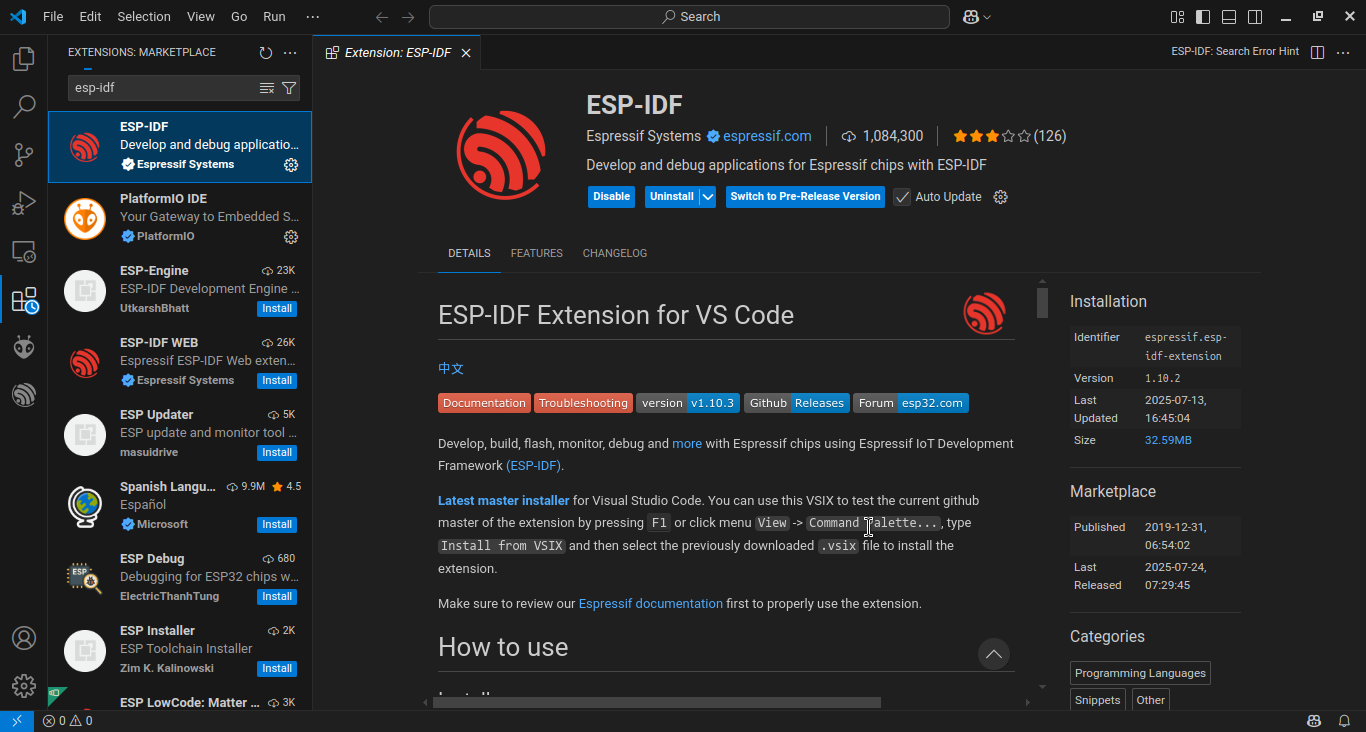
\includegraphics[scale=0.2]{img/VSCodeESP-IDF.png}
    \label{fig:VSCodeESPIDF}
\end{figure}

A janela de configuração apresentada será uma igual ao da Figura
\ref{fig:ESPIDFConfig}. Para a simplicidade do usuário, será
utilizado o modo \textit{Express} da configuração do ambiente.
Ao apertar no botão \textit{Express} aparecerá uma nova janela
como na Figura \ref{fig:ESPIDFConfigExpress}.

\begin{figure}[!ht]
    \centering
    \caption{Página de Configuração do ESP-IDF}
    \vspace{0.2cm}
    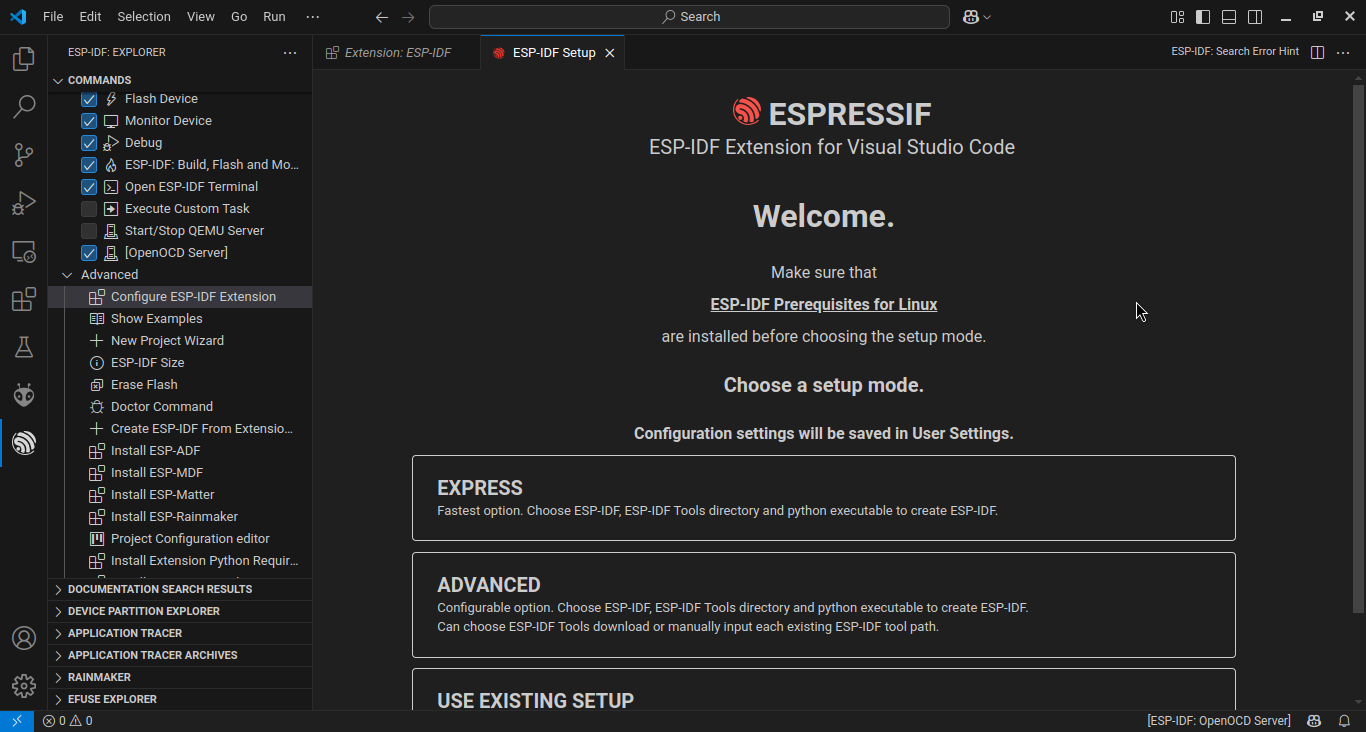
\includegraphics[scale=0.2]{img/VSCodeESP-IDF_CONFIGURE.png}
    \label{fig:ESPIDFConfig}
\end{figure}

Na janela da Figura \ref{fig:ESPIDFConfigExpress}, seleciona a versão
que deseja para a ESP-IDF (sempre é melhor selecionar a versão do
github para ficar a mais atualizada); especifique a localização que
será instalado o sistema; e por fim a localização de onde está
instaldo o Python (geralmente o programa identifica no sistema).

\begin{figure}[!ht]
    \centering
    \caption{Página de configuração na janela \textit{Express}}
    \vspace{0.2cm}
    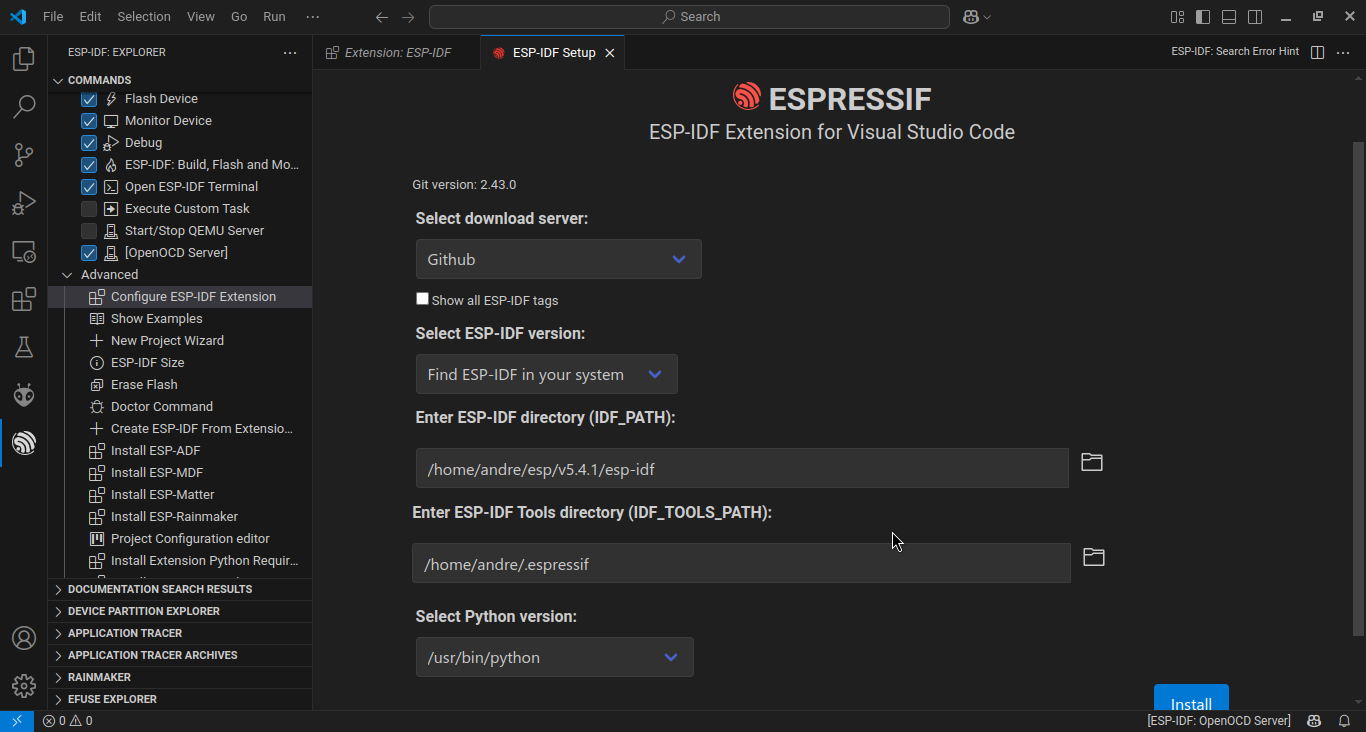
\includegraphics[scale=0.2]{img/VSCodeESP-IDF_CONFIGURE_02.png}
    \label{fig:ESPIDFConfigExpress}
\end{figure}

%===============================================
\subsection{Putty}

\tab
Para salvar os dados em um arquivo no sistema 
operacional \textbf{Windows}, necessita instalar o 
programa \href{https://www.chiark.greenend.org.uk/~sgtatham/putty/latest.html}{Putty}.
Seguindo a instalação corretamente, aparecerá uma janela
como a da figura seguinte.

% Tirar foto das janelas do putty